\section{HexGrid}
\label{sec:hexgrid}

The HexGrid class is, as the name suggests, a general class for managing every instance of hexagonal grids in the game, which includes the editor and the board. The constructor of HexGrid takes various parameters, like the size of the grid, the size of each tile including information on the angles, in case the tile is not a perfect hexagon, as well as the grid's position on the screen. After construction, an instance of HexGrid provides several useful functions described in this section.

\subsection{Checking if a Position is Inside Grid}
Internally, the hexagonal grid is represented by a square array. Using this representation, however, some of the elements of the array is not part of the grid, as seen in \autoref{fig:hexgrid_array}. Because of this, a functionality is needed to check whether position, given in x and y coordinates of the array, is actually inside the grid. The \texttt{is\_inside} function of the HexGrid prototype does just that.

\begin{figure}[ht]
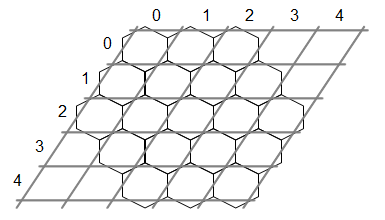
\includegraphics[scale=1]{img/hexgrid_array.png}
\caption{Array representation of a hexagonal grid (edge size 3)}
\label{fig:hexgrid_array}
\end{figure}

The functions start by sorting out things that are out of array bounds, both negative and too large coordinate numbers simple result in the function returning \texttt{false}. It then calculates the difference between the x and y coordinate of the input. If this number is larger than or equal to the edge size of the grid, it means that the position is in one of the ``corners'' of the square array that does not represent a tile, as shown in \autoref{fig:hexgrid_array}.

\subsection{Calculating the Screen Point of a Tile}
When you have to draw the grid, you need to find out where on the screen a given tile should be located. The \texttt{get\_pixel\_coordinate} function is used for this purpose. This function is actually very simple. During the constructor, 2 values were calculated, \texttt{delta\_x} and \texttt{delta\_x}. Each of these are a 2 dimensional vector, representing the screen distance moved whenever 1 is added to the tile x and y respectively. The tile x coordinate is multiplied with the \texttt{delta\_x}, and the tile y coordinate is multiplied with the \texttt{delta\_y}, and the two resulting vectors are added together. Finally, the the origin, which is the center of the \texttt{(0,0)} tile on screen is added to the result of the first addition, and the result is the center of the desired tile.

\subsection{Calculating the Tile Position of a Pixel Point}
The functionality of converting a pixel coordinate to a tile position is needed as well. An example of this, is having to detect which tile was clicked in the program editor, when knowing only the mouse position. The function \texttt{get\_tile\_position} serves this purpose, and the calculation is a bit more involved than going the other way around. The chosen way of implementing this is using two points, called low and high which both start set to the origin. Then the \texttt{delta\_y} vector is added to or subtracted form each of these a number of times, so that the high point has the lowest possible y-coordinate that is higher than the input y-coordinate, and the low is at the highest possible y-coordinate that is lower than the input y-coordinate. The number of steps are counted for each.

Considering that the grids used in this game have horizontal rows of tiles, it is clear that at this point, the low and high points can be moved along the \texttt{delta\_x} axis and still bound the y-coordinate of the input. Therefore, at this point the \texttt{delta\_x} is added to or subtracted from each point a number of times that gives the tightest possible x-coordinate bound around the input, counting the steps taken. At this point low and high are adjacent, but never in the same horizontal row, and one of them are center of the tile which was clicked.

The final step of the calculation is using the information about the angle of the edges on the tile, to generate the line representing the border between the high and low tile. If the input point is above the line, high is the correct point, else low is correct. Using the step counts of the correct tile, the position of the desired tile in the grid array is \texttt{(delta\_x steps , delta\_y steps)}, which is returned.